% =============================================================================
% Lecture 12b: Benchmarking, Part 2 (Deciding from Measurements)
% Introduction to Machine Learning Systems (Volume I)
% =============================================================================
% A measurement supports a decision only when the difference exceeds its noise,
% the comparison changes one thing at a time, the score has not become the
% target, and the model keeps its quality on the frontier and against gates
% fixed before the test.
%
% Build: make -C slides build-12b_benchmarking   (figures: images/make_figs.py)
% Plan:  lecture_map.yml and storyboard.md in this folder.
% =============================================================================

\documentclass[aspectratio=169, 12pt]{beamer}
\usepackage{../../assets/beamerthememlsys}
\mlsyssetup{
  volume={Volume I},
  chapter={Chapter 12},
  chaptertitle={Benchmarking, Part 2},
  logo={../../assets/img/logo-mlsysbook.png},
  instlogo={../../assets/img/logo-harvard.png},
  layer=hardware,
  dividerstack,
}
\usepackage[T1]{fontenc}
\usepackage[scaled=0.9]{helvet}
\usepackage{courier}
\renewcommand{\familydefault}{\sfdefault}
\usepackage{booktabs,amsmath}
\graphicspath{{images/}}
% Generated by calcs.py. Do not edit; edit calcs.py and rerun it.
\defval{eos_score}{13.33}
\defval{dell_score}{13.22}
\defval{hook_gap_pct}{0.8}
\defval{dell_spread}{0.02}
\defval{eos_spread}{0.13}
\defval{target_top1}{75.9}
\defval{epochs}{35}
\defval{scale_factor}{1.0042}
\defval{dell_fail_top1}{75.894}
\defval{dell_fail_frac}{0.75894}
\defval{n_runs}{20}
\defval{n_systems}{4}
\defval{recall_tops}{10}
\defval{recall_w}{0.5}
\defval{recall_sus_tops}{3}
\defval{recall_sus_w}{2}
\defval{recall_eff}{20}
\defval{recall_sus_eff}{1.5}
\defval{log_seed}{5675}
\defval{global_batch}{3200}
\defval{ev_first_frac}{0.29274}
\defval{ev_first_epoch}{3}
\defval{ev_between}{7}
\defval{ev_every}{4}
\defval{ev_last_epoch}{35}
\defval{log_eos_frac}{0.75936}
\defval{log_eos_top1}{75.936}
\defval{log_eos_ms}{798{,}372}
\defval{log_eos_min}{13.3062}
\defval{cv_eos}{0.48}
\defval{cv_dell}{0.06}
\defval{cv_h200}{0.07}
\defval{cv_n8}{0.04}
\defval{eos_span}{0.99}
\defval{eos_span_int}{1}
\defval{others_span}{0.2}
\defval{dell_fail_pct}{6.0}
\defval{n8_fail_pct}{5.4}
\defval{cv_ratio}{7.5}
\defval{rtx_cv}{2.2}
\defval{acc_lo}{75.88}
\defval{acc_hi}{76.21}
\defval{acc_spread}{0.32}
\defval{acc_spread_eos}{0.31}
\defval{acc_mean_int}{76}
\defval{val_images}{50{,}000}
\defval{binom_hw}{0.37}
\defval{dell_fail_min}{13.94}
\defval{dell_middle}{13.163}
\defval{z95}{1.96}
\defval{z99}{2.576}
\defval{acc_p}{0.95}
\defval{acc_p_pct}{95}
\defval{acc_q}{0.05}
\defval{acc_m}{0.01}
\defval{acc_m_pts}{1}
\defval{acc_conf}{95}
\defval{p90_p}{0.90}
\defval{p90_m}{0.005}
\defval{p90_m_pts}{0.5}
\defval{p99_p}{0.99}
\defval{p99_m}{0.0005}
\defval{p99_m_pts}{0.05}
\defval{q_conf}{99}
\defval{n_acc}{1{,}825}
\defval{n_p90}{23{,}886}
\defval{n_p99}{262{,}742}
\defval{min_p90}{24{,}576}
\defval{min_p99}{270{,}336}
\defval{edge_share_pct}{5}
\defval{eos_n}{5}
\defval{dell_n}{4}
\defval{n_conv_words}{nine}
\defval{eos_mean}{13.263}
\defval{eos_mean_short}{13.26}
\defval{eos_sd}{0.063}
\defval{dell_mean}{13.159}
\defval{dell_sd}{0.0084}
\defval{d_dell}{0.104}
\defval{se_dell}{0.0285}
\defval{t_dell}{2.73}
\defval{dof_dell}{4.2}
\defval{lo_dell}{0.026}
\defval{hi_dell}{0.182}
\defval{lo_dell_short}{0.03}
\defval{hi_dell_short}{0.18}
\defval{d_h200}{1.235}
\defval{se_h200}{0.0285}
\defval{t_h200}{2.74}
\defval{lo_h200}{1.16}
\defval{hi_h200}{1.31}
\defval{eq_hw}{0.10}
\defval{pct_dell}{0.8}
\defval{pct_lo_dell}{0.2}
\defval{pct_hi_dell}{1.4}
\defval{pct_dellall}{-0.4}
\defval{pct_lo_dellall}{-3.7}
\defval{pct_hi_dellall}{2.9}
\defval{pct_h200}{9.3}
\defval{pct_lo_h200}{8.7}
\defval{pct_hi_h200}{9.9}
\defval{pct_lo_dellall_abs}{3.7}
\defval{pct_h200_int}{9}
\defval{min_useful}{2}
\defval{hw_5}{0.59}
\defval{hw_10}{0.34}
\defval{hw_20}{0.22}
\defval{res_diff}{0.5}
\defval{res_runs}{15}
\defval{res_runs_one}{4}
\defval{z_power}{0.84}
\defval{vote_base}{95}
\defval{vote_comp}{94}
\defval{vote_n}{1{,}000}
\defval{vote_err_base}{50}
\defval{vote_err_comp}{60}
\defval{vote_lo_abs}{1}
\defval{vote_hi}{3}
\defval{vote_gap}{10}
\defval{chi2}{3.84}
\defval{vote_max}{26}
\defval{best_run}{2}
\defval{worst_run}{4}
\defval{best_top1}{76.206}
\defval{worst_top1}{75.900}
\defval{seed_gap}{153}
\defval{seed_max}{6{,}093}
\defval{seed_max_pct}{12}
\defval{sys_dell_diff}{30}
\defval{sys_dell_all}{44}
\defval{sys_h200_diff}{7}
\defval{sys_h200_all}{44}
\defval{container_gap}{seven}
\defval{h200_bw}{4.8}
\defval{h100_bw}{3.35}
\defval{h200_bw_more}{43}
\defval{h200_sparse}{1{,}979}
\defval{lee_start}{2.4}
\defval{lee_end}{3.9}
\defval{order_blocked}{20}
\defval{order_inter}{4}
\defval{beam_w0}{1}
\defval{beam_w1}{10}
\defval{beam_gain}{0.5}
\defval{beam_lat0}{50}
\defval{beam_lat1}{200}
\defval{beam_slo}{100}
\defval{beam_ratio_words}{ten}
\defval{beam_slow_words}{four}
\defval{s4_gfx}{37.9}
\defval{s4_glb}{43.2}
\defval{s4_gain}{14}
\defval{s4_game_mhz}{480}
\defval{s4_bench_mhz}{532}
\defval{s4_max_mhz}{533}
\defval{recht_models}{64}
\defval{recht_lo}{10.3}
\defval{recht_hi}{13.6}
\defval{recht_rho}{0.997}
\defval{gsm1k_drop}{8}
\defval{sd_mobilenetv1_top1}{70.6}
\defval{sd_mobilenetv1_ms}{113}
\defval{sd_mobilenetv2_top1}{72.0}
\defval{sd_mobilenetv2_ms}{75}
\defval{sd_nasneta_top1}{74.0}
\defval{sd_nasneta_ms}{183}
\defval{sd_mobilenetv214_top1}{74.7}
\defval{sd_mobilenetv214_ms}{143}
\defval{frame_budget}{33}
\defval{chu_top1_lo}{75.1}
\defval{chu_top1_hi}{76.2}
\defval{chu_v3_cpu}{20.3}
\defval{chu_v1_cpu}{54.7}
\defval{chu_v1_dsp}{3.72}
\defval{chu_v3_dsp}{4.51}
\defval{bin1_n}{20}
\defval{bin1_conf}{0.65}
\defval{bin1_acc_pct}{60}
\defval{bin1_gap}{0.05}
\defval{bin1_w}{0.2}
\defval{bin2_n}{30}
\defval{bin2_conf}{0.85}
\defval{bin2_acc_pct}{80}
\defval{bin2_gap}{0.05}
\defval{bin2_w}{0.3}
\defval{bin3_n}{50}
\defval{bin3_conf}{0.97}
\defval{bin3_acc_pct}{84}
\defval{bin3_gap}{0.13}
\defval{bin3_w}{0.5}
\defval{bins_total}{100}
\defval{ece}{0.09}
\defval{alert_conf}{85}
\defval{guo_lenet_err}{44.9}
\defval{guo_resnet_err}{30.6}
\defval{guo_lenet_ece}{4.85}
\defval{guo_resnet_ece}{16.53}
\defval{guo_in_ece}{5.48}
\defval{guo_in_ece_ts}{1.86}
\defval{guo_ratio}{3.4}
\defval{wilds_id_acc}{75.7}
\defval{wilds_ood_acc}{71.6}
\defval{wilds_id_f1}{47.0}
\defval{wilds_ood_f1}{31.0}
\defval{wilds_acc_drop}{4.1}
\defval{wilds_f1_drop}{16.0}
\defval{wilds_acc_drop_int}{4}
\defval{wilds_f1_drop_int}{16}
\defval{wilds_reps}{3}
\defval{camelyon_id}{93.2}
\defval{camelyon_ood}{70.3}
\defval{g_top1_fp32}{71.8}
\defval{g_top1_int8}{70.9}
\defval{g_top5_fp32}{91}
\defval{g_top5_int8}{90.4}
\defval{g_ece_fp32}{0.031}
\defval{g_ece_int8}{0.089}
\defval{g_edge_fp32}{68.2}
\defval{g_edge_int8}{61.4}
\defval{g_edge_fp32_int}{68}
\defval{g_limit}{1}
\defval{g_limit_words}{one}
\defval{g_top1_loss}{0.9}
\defval{g_edge_drop}{6.8}
\defval{g_test}{1{,}000}
\defval{g_edge_n}{50}
\defval{g_edge_hw}{13}
\defval{img_w}{224}
\defval{img_h}{224}
\defval{img_c}{3}
\defval{img_bits}{8}
\defval{img_levels}{256}
\defval{img_values}{150{,}528}
\defval{space_exp}{362{,}508}
\defval{test_n}{50{,}000}
\defval{test_exp}{4.7}
\defval{frac_exp}{362{,}503}

\setcounter{mlsystotalsections}{4}

\title{Benchmarking, Part 2}
\author{Vijay Janapa Reddi}
\institute{Harvard University}
\date{}

% A large answer choice for predict and concept-question slides
\newcommand{\choice}[2]{\textbf{\textcolor{mlsysaccent}{#1}}\enspace #2}
% A highlighted answer choice from overlay #1 on
\newcommand{\choicehl}[3]{\alt<#1->{\colorbox{mlsysaccent!15}{\choice{#2}{#3}}}{\choice{#2}{#3}}}
% A goal or takeaway line with its thumbnail
\newcommand{\thumbline}[2]{%
  \begin{minipage}[c]{2.6cm}\centering\includegraphics[width=2.5cm,height=1.05cm,keepaspectratio]{#1}\end{minipage}%
  \hspace{0.3cm}\begin{minipage}[c]{0.74\textwidth}\normalsize #2\end{minipage}}
% A condition or verdict tag
\newcommand{\condtag}[2]{\colorbox{#1!12}{\parbox{3.9cm}{\centering\footnotesize\textbf{\textcolor{#1}{#2}}}}}
% A table cell that differs from Eos, highlighted from overlay #1 on
\newcommand{\diffcell}[2]{\alt<#1->{\colorbox{RedLine!15}{\textbf{#2}}}{#2}}
% One line of a quoted log or tool output, in monospace
\newcommand{\logline}[1]{#1\\}
% A block of quoted log or tool output: monospace, tight lines
\newenvironment{logblock}{\par\ttfamily\scriptsize\raggedright\setlength{\parskip}{0pt}\setlength{\baselineskip}{10.5pt}}{\par}
% A highlighted key inside a quoted log line
\newcommand{\logkey}[2]{{\setlength{\fboxsep}{1pt}\colorbox{#1!15}{#2}}}
% A line of a worked calculation shown from overlay #1 on
\newcommand{\calcline}[2]{\uncover<#1->{#2}\\[0.12cm]}


\begin{document}

% =============================================================================
% TITLE, HOOK, RECALL
% =============================================================================
\mlsysnote{[0.5 min] Read the thesis aloud once. Part 1 asked what a benchmark number must state before it is a test. Today asks what to do when two numbers disagree. Is the difference real, is it the difference we meant to measure, has the score stopped measuring, and does the model still pass? The notes total about 71.5 minutes. FLEX: cutting the frames tagged [OPTIONAL] leaves a complete lecture of about 49.5 minutes.}
\mlsystitle{Benchmarking, Part~2}{A measurement supports a decision only when the difference exceeds its noise, one thing changed, the score is not the target, and the model clears gates set before the test.}{cover_benchmarking_blueprint.png}

\begin{frame}{Predict: is one eight-H100 server faster than the other?}
  \mlsysactivity{Predict}{2 min}
  \centering
  \mlsyssteps[width=0.95\textwidth,height=5.0cm,keepaspectratio]{hook_step}{2}\\[0.1cm]
  {\normalsize\choice{A}{yes, by \val{hook_gap_pct}\%}\qquad\choice{B}{no, the gap is noise}\qquad\choicehl{2}{C}{these two numbers cannot say}}
  \mlsyscredit{MLCommons, MLPerf Training v4.0, closed, ResNet-50: Dell XE9680x8H100-SXM-80GB and NVIDIA eos\_ngc24.04\_mxnet, result\_0 to result\_4. Score: mean of the middle three runs $\times$ \val{scale_factor} (scaling.json).}
  \note{[3 min] LINK: Part 1 ended on MLPerf, the suite that fixes the model, the data, and the quality target. Step 1: two published MLPerf Training results from June 2024. Each server has eight H100 accelerators, and each trained ResNet-50 on ImageNet until it reached \val{target_top1} percent top-1. Dell's score is \val{dell_score} minutes; NVIDIA's Eos server scored \val{eos_score} minutes. ENGAGE: is Dell's server faster? Vote with fingers, A, B, or C. Step 2: C. Each bar is a score computed from five runs, and the decision needs the runs. Point to the strip. Dell's four converged runs sit within \val{dell_spread} minutes of each other. Its fifth run trained all \val{epochs} epochs and stopped at \val{dell_fail_top1} percent, just short of the target. Eos's five runs spread over \val{eos_spread} minutes. Students who chose A treated a score as a measurement without noise. Students who chose B guessed a conclusion that segment 2 overturns. The published score is a trimmed mean of the runs, explained in segment 1. Ask: what would you need to decide? FLEX: [CORE].}
\end{frame}

\begin{frame}{Recall: what must a benchmark number state?}
  \mlsysactivity{Retrieval}{1.5 min}
  \begin{columns}[c]
    \begin{column}{0.40\textwidth}
      \centering\safeimg[width=\textwidth,height=3.0cm,keepaspectratio]{recall_hook.pdf}\\[0.1cm]
      {\footnotesize Lecture 12's hook: \val{recall_eff} against \val{recall_sus_eff} TOPS/W.}
    \end{column}
    \begin{column}{0.56\textwidth}
      \centering
      \only<1|handout:0>{{\Large\bfseries Close your notes.}\\[0.3cm]{\normalsize Name four conditions a benchmark number must state before it is a test.}}%
      \only<2-|handout:1>{%
        \condtag{BlueLine}{Load and statistic}\\[0.12cm]
        \condtag{BlueLine}{Boundary: what is timed}\\[0.12cm]
        \condtag{OrangeLine}{Scenario: how queries arrive}\\[0.12cm]
        \condtag{OrangeLine}{Power boundary and heat}\\[0.25cm]
        \condtag{midgray}{Today: the noise}\\[0.12cm]
        \condtag{midgray}{Today: the quality held}}
    \end{column}
  \end{columns}
  \mlsyscredit{Lecture 12 (Benchmarking, Part 1); hook values illustrative, Benchmarking \S12.7.}
  \note{[1.5 min] ENGAGE: close your notes, one minute, write the four conditions from Lecture 12. Step 2: the load and the statistic, such as p99 latency (the time 99 percent of requests beat) under open-loop arrivals; the boundary, from one kernel to end to end; the scenario, such as SingleStream against Offline; and the power boundary with its thermal state and duty cycle. Those four made ``\val{recall_tops} TOPS at \val{recall_w} W'' (trillions of operations per second) into \val{recall_sus_eff} TOPS per watt. Today adds the last two: the noise around a number, and the quality the model held. FLEX: [CORE]; if students have not seen Part 1, read the four tags aloud and move on.}
\end{frame}

\begin{frame}{Two measurements disagree: how do we decide?}
  \centering
  {\normalsize Is the difference real, is it the one we meant to measure,\\and can the model ship?}\\[0.2cm]
  \raggedright
  \thumblinesm[\normalsize]{thumb_strip_step2.pdf}{Size the noise in a benchmark, and the runs and samples a number needs.}\\[0.16cm]
  \thumblinesm[\normalsize]{thumb_interval_step5.pdf}{Put an interval on a difference, change one thing, and set a threshold first.}\\[0.16cm]
  \thumblinesm[\normalsize]{thumb_recht.pdf}{Recognize a score that has become the target, and the rules that defend it.}\\[0.16cm]
  \thumblinesm[\normalsize]{thumb_ece_step3.pdf}{Accept a model on its frontier, calibration, slices, and gates.}\par\vspace{0.2cm}
  \threadstrip{1}{0}{0}{0}{0}
  \note{[1.5 min] The driving question and four goals, one per segment. Two running examples carry the lecture. The system half is real: \val{n_runs} published MLPerf Training runs from four submissions, the two servers in the hook plus an eight-H200 server and a 64-GPU Eos system. The model half is the chapter's camera trap: an INT8 MobileNetV2 against its FP32 original, made concrete with published measurements of calibration and of camera traps a model has never seen. Tell students the deck returns to the hook's dot strip at the end, with three verdicts. The strip fills the right half of the dual mandate: today decides whether a difference, and a model, can be trusted. FLEX: [CORE].}
\end{frame}

% =============================================================================
% SECTION: NOISE
% =============================================================================
\mlsysnote{[0.5 min] First, measure the noise itself. Run the same code on the same machine five times and the answers differ. How much, and what does a suite do about it? FLEX: [CORE].}
\mlsysdivider{How much does a benchmark move when nothing changes?}{Benchmarking, \S12.4.2, \S12.8.1, \S12.8.2}
\section{Noise}

\begin{frame}[t]{Each run's log records its seed, its accuracy, and its fate}
  \raggedright
  {\footnotesize\textbf{NVIDIA Eos, 8 $\times$ H100:} {\scriptsize\texttt{resnet/result\_0.txt}}, 347 lines\par}\vspace{0.08cm}
  \begin{logblock}
  \logline{:::MLLOG \{... "key": \logkey{BlueLine}{"seed", "value": \val{log_seed}}, ...\}}
  \logline{:::MLLOG \{... "key": "global\_batch\_size", "value": \val{global_batch}, ...\}}
  \logline{:::MLLOG \{... "time\_ms": \logkey{OrangeLine}{1714042844981}, ... "key": "run\_start", ...\}}
  \logline{:::MLLOG \{... "key": "eval\_accuracy", "value": \val{ev_first_frac}, ... "epoch\_num": \val{ev_first_epoch}\}\}}
  \logline{\textsf{\textcolor{midgray}{\quad \val{ev_between} more evaluations, one every \val{ev_every} epochs}}}
  \logline{:::MLLOG \{... "key": \logkey{GreenLine}{"eval\_accuracy", "value": \val{log_eos_frac}}, ... "epoch\_num": \val{ev_last_epoch}\}\}}
  \logline{:::MLLOG \{... "time\_ms": \logkey{OrangeLine}{1714043643353}, ... "key": "run\_stop", ...}
  \logline{\ \ \ \ ... \logkey{GreenLine}{"status": "success"}, "epoch": 34\}\}}
  \end{logblock}
  \vspace{0.12cm}
  {\footnotesize\textbf{Dell XE9680, 8 $\times$ H100:} {\scriptsize\texttt{resnet/result\_4.txt}}, the last two lines\par}\vspace{0.08cm}
  \begin{logblock}
  \logline{:::MLLOG \{... "key": \logkey{RedLine}{"eval\_accuracy", "value": \val{dell_fail_frac}}, ... "epoch\_num": \val{ev_last_epoch}\}\}}
  \logline{:::MLLOG \{... "key": "run\_stop", ... \logkey{RedLine}{"status": "aborted"}, "epoch": 36\}\}}
  \end{logblock}
  \vspace{0.08cm}
  \uncover<2->{\footnotesize \texttt{run\_stop} $-$ \texttt{run\_start} $=$ \val{log_eos_ms} ms $=$ \val{log_eos_min} min: one dot of the next slide.}
  \mlsyscredit{MLCommons training\_results\_v4.0 (Apache 2.0), NVIDIA/results/eos\_ngc24.04\_mxnet and Dell/results/XE9680x8H100-SXM-80GB; fields elided (...). Minutes derived.}
  \note{[2 min] NARRATE: every MLPerf number on today's slides comes from files like these, public on GitHub. Each run writes one log; each line is a JSON event after the marker MLLOG. Point to the blue key: the random seed, a different one for every run, which sets the initial weights and the data order. The batch size is fixed by the submission. Step 2: the timer is the two orange timestamps. run\_stop minus run\_start is \val{log_eos_ms} milliseconds, \val{log_eos_min} minutes, and that is this run's dot on the next slide. Green: the last evaluation reached \val{log_eos_top1} percent and the status reads success. Below, Dell's fifth run evaluated \val{dell_fail_top1} percent at epoch \val{ev_last_epoch}, missed \val{target_top1}, and stopped at epoch 36 with status aborted. That one word is why the hook's Dell score drops a run. ENGAGE: which line would you check first if a published score looked too good? Expected: the status and the last eval\_accuracy of every run, then the seeds, which the rules require to come from the clock or the system's random source, never chosen by hand. WARN: students assume a benchmark score is measured once. It is computed from several logs by a rule, and the logs are the evidence. FLEX: [OPTIONAL]; cutting it loses the real run log.}
\end{frame}

\begin{frame}{Identical runs of one server differ by up to \val{eos_span_int} percent}
  \centering
  \mlsyssteps[width=0.95\textwidth,height=4.8cm,keepaspectratio]{strip_step}{2}\\[0.1cm]
  \uncover<3->{\small Sources: \textbf{machine} (clocks, OS jitter) \quad \textbf{algorithm} (seed, data order) \quad \textbf{sample} (finite test set)}
  \mlsyscredit{MLPerf Training v4.0 closed, ResNet-50, four submissions, \val{n_runs} runs (result\_0 to result\_4). CV over converged runs, derived.}
  \note{[3 min] Step 1: all \val{n_runs} runs, one row per submission, each run placed relative to its own system's median, so the four rows share one axis. Eos's five runs span \val{eos_span} percent of its run time. The other three systems sit within about \val{others_span} percent. Two runs, one Dell and one on the 64-GPU Eos system, did not reach \val{target_top1} percent; they are off the scale at \val{dell_fail_pct} and \val{n8_fail_pct} percent slower. Step 2: the coefficient of variation (CV), the standard deviation divided by the mean, for the converged runs: \val{cv_eos} percent for Eos, \val{cv_dell} for Dell, \val{cv_h200} for H200, \val{cv_n8} for 64 GPUs. Step 3: the chapter's three sources of noise: the machine (clocks, interrupts, temperature), the algorithm (seed, data order, reduction order), and the sample (a finite test set). ENGAGE: these runs used the same code and hardware; why would one system be \val{cv_ratio} times noisier than another? Expected: we cannot tell from the logs; the chapter's point is to measure the spread. WARN: the chapter gives no universal cutoff such as 5 percent CV (Perspective 12.4); report the CV and judge it against the difference you want to detect. Example: a 2026 preprint measured LLM decoding at \val{rtx_cv} percent CV on an RTX 4050 laptop (Tummalapalli et al.). FLEX: [CORE].}
\end{frame}

\begin{frame}{Within one recipe, seeds move accuracy by a third of a point}
  \centering
  \mlsyssteps[width=0.95\textwidth,height=5.1cm,keepaspectratio]{seedacc_step}{2}
  \mlsyscredit{MLPerf Training v4.0 logs (last eval\_accuracy, \val{n_runs} runs, one seed each). Binomial 95\% half-width at \val{acc_mean_int}\% on \val{val_images} images, derived.}
  \note{[2.5 min] The same \val{n_runs} runs, now by accuracy at their last evaluation. Each run used a different random seed; the code, data, and hyperparameters are fixed within a submission. Step 1: top-1 ranges from \val{acc_lo} to \val{acc_hi} percent, and two runs landed just under the \val{target_top1} percent target. Step 2: the spread across all \val{n_runs} runs is \val{acc_spread} points; Eos's five runs alone span \val{acc_spread_eos}, so one recipe moves by about a third of a point. Data order and reduction order vary with the seed too. Below it is the second source of noise; a test set is a sample. A different draw of \val{val_images} images would move a \val{acc_mean_int} percent accuracy by about plus or minus \val{binom_hw} points at 95 percent, from the binomial formula on the next slides. Define the term once: a 95 percent interval is one built so that, over many repeats of the experiment, 95 of 100 such intervals contain the true value. ENGAGE: a paper reports a 0.2-point gain from one run of each model. What can it claim? Expected: nothing yet; the gain is smaller than this recipe's own seed spread. LINK: in the chapter, seeds reverse deep reinforcement learning results (Henderson et al. 2018) and GAN rankings (Lucic et al. 2018). FLEX: [OPTIONAL]; cutting it loses the seed-to-seed spread.}
\end{frame}

\begin{frame}{MLPerf drops the fastest and slowest run, then averages}
  \centering
  \mlsyssteps[width=0.95\textwidth,height=3.5cm,keepaspectratio]{olympic_step}{3}\\[0.02cm]
  {\footnotesize\textit{``Each benchmark result is computed by dropping the fastest and slowest runs, then taking the mean of the remaining times. For this purpose, a single non-converging run may be treated as the slowest run and dropped.''}}\\[0.05cm]
  \uncover<3->{\small Published score: $\val{dell_middle} \times \val{scale_factor} = \val{dell_score}$ min.}
  \mlsyscredit{Quoted: mlcommons/training\_policies, training\_rules.adoc, Scoring (commit 9f32f97, April 2024). Dell runs: MLPerf Training v4.0.}
  \note{[2.5 min] The suite applies statistics to itself; read the quoted rule aloud. The rules require at least five runs, and a second non-converging run invalidates the result. Step 1: Dell's five runs, sorted. Run 5 is far to the right: \val{dell_fail_min} minutes, and it never reached \val{target_top1} percent. Step 2: the rule drops the fastest run and the slowest. A run that misses the target counts as the slowest, so it is the one dropped at the top. Step 3: the mean of the middle three is \val{dell_middle} minutes. The published score multiplies by \val{scale_factor}, a factor the review committee set because these runs converged in fewer epochs than the reference implementation; every ResNet score in the round carries it. ENGAGE: why drop both ends instead of reporting the best run? Expected: this trimmed mean resists one lucky run and one stalled run. Why count a failed run as the slowest? Expected: time to quality includes the risk of not reaching quality. WARN: running many sets of five and submitting the best set is forbidden. The rules allow a sliding window of N consecutive runs from M chosen in advance, submitting the median window. FLEX: [OPTIONAL]; cutting it loses MLPerf's scoring rule.}
\end{frame}

\begin{frame}[t]{Estimate: how many samples does a number need?}
  \mlsysactivity{Estimate}{2.5 min}
  \centering
  {\large $n = \dfrac{z^2\, p\,(1-p)}{m^2}$}\quad
  {\footnotesize $p$: fraction that passes;\; $m$: margin;\; $z$: \val{z95} at \val{acc_conf}\%, \val{z99} at \val{q_conf}\%}\\[0.15cm]
  \small
  \begin{tabular}{@{}lccccr@{}}
    \toprule
    \textbf{Claim} & $p$ & $m$ & \textbf{Confidence} & $n$ & \textbf{MLPerf} \\
    \midrule
    Accuracy \val{acc_p_pct}\% $\pm$ \val{acc_m_pts} point & \val{acc_p} & \val{acc_m} & \val{acc_conf}\% & \uncover<2->{\textbf{\val{n_acc}}} & \\
    p90: share under bound $\pm$ \val{p90_m_pts} points & \val{p90_p} & \val{p90_m} & \val{q_conf}\% & \uncover<3->{\textbf{\val{n_p90}}} & \uncover<3->{\val{min_p90}} \\
    p99: share under bound $\pm$ \val{p99_m_pts} points & \val{p99_p} & \val{p99_m} & \val{q_conf}\% & \uncover<3->{\textbf{\val{n_p99}}} & \uncover<3->{\val{min_p99}} \\
    \bottomrule
  \end{tabular}\\[0.15cm]
  \uncover<4->{\safeimg[width=0.85\textwidth,height=1.95cm,keepaspectratio]{sizing.pdf}}
  \mlsyscredit{Benchmarking, Napkin Math 12.5 (\val{n_acc} images). MLPerf Inference rules, minimum query counts (mlcommons/inference\_policies). $n$ derived.}
  \note{[3 min] An accuracy and a latency percentile are the same kind of number: the fraction of trials that pass. Define each term: p is that fraction, m the margin we want, z the number of standard errors for the confidence level. ENGAGE: one minute with a neighbor. How many test images pin a \val{acc_p_pct} percent accuracy to within one point at \val{acc_conf} percent confidence? Step 2: \val{z95} squared times \val{acc_p} times \val{acc_q}, over \val{acc_m} squared: about \val{n_acc} images, the chapter's number. Step 3: MLPerf Inference applies the same formula to the 90th percentile at \val{q_conf} percent confidence and a \val{p90_m_pts} percent margin: \val{n_p90} queries, which the rules round up to \val{min_p90}. The 99th percentile with a \val{p99_m_pts} percent margin needs \val{n_p99}, rounded to \val{min_p99}. The margin is on the percentile's rank, not on the latency in milliseconds. Step 4: on a log scale, the deep tail costs more than 100 times the accuracy estimate. WARN: a test set sized for one accuracy number is far too small for a slice that is \val{edge_share_pct} percent of it; segment 4 returns to this. MLPerf's early-stopping rule lets a system far inside its latency bound stop sooner, at a small penalty. LINK: Lecture 13 explains how queues create the tail this run measures. FLEX: [CORE].}
\end{frame}

% =============================================================================
% SECTION: FAIR COMPARISON
% =============================================================================
\mlsysnote{[0.5 min] Now the hook's question. A difference is a finding when it is larger than its noise, it is attributable when one thing changed, and it is worth acting on when it clears a threshold set before the test. FLEX: [CORE].}
\mlsysdivider{Is the difference real, and is it the one we meant to measure?}{Benchmarking, \S12.8.1, \S12.2.6, \S12.8.3}
\section{Fair Comparison}

\begin{frame}[t]{The hook's gap is larger than its noise: \val{lo_dell_short} to \val{hi_dell_short} minutes}
  \begin{columns}[T]
    \begin{column}{0.46\textwidth}
      \raggedright\footnotesize
      \textbf{Given:} raw times, converged runs\\
      \textcolor{midgray}{(Score: middle-three mean $\times$ \val{scale_factor})}\\[0.08cm]
      Eos: \val{eos_n} runs, mean \val{eos_mean}, SD \val{eos_sd}\\
      Dell: \val{dell_n} runs, mean \val{dell_mean}, SD \val{dell_sd}\\[0.12cm]
      \calcline{2}{1. $d = \val{eos_mean} - \val{dell_mean} = \val{d_dell}$ min}
      \calcline{3}{2. $\text{SE} = \sqrt{\val{eos_sd}^2/\val{eos_n} + \val{dell_sd}^2/\val{dell_n}} = \val{se_dell}$}
      \calcline{4}{3. $\val{d_dell} \pm \val{t_dell} \times \val{se_dell}$: \val{lo_dell} to \val{hi_dell}}
      \calcline{5}{4. H200: $\val{d_h200} \pm \val{t_h200} \times \val{se_h200}$: \val{lo_h200} to \val{hi_h200}}
    \end{column}
    \begin{column}{0.52\textwidth}
      \centering
      \mlsyssteps[width=\textwidth,height=5.75cm,keepaspectratio]{interval_step}{5}
    \end{column}
  \end{columns}
  \mlsyscredit{MLPerf Training v4.0 logs; Welch interval (95\%, $t$ at about \val{dof_dell} degrees of freedom), derived. Rule for reading it: Benchmarking, \S12.8.1.}
  \note{[5 min] Step 1: the hook's \val{n_conv_words} converged runs, raw times, each mean a black bar. The hook's scores differ, since a score is the middle-three mean times \val{scale_factor}, so Eos's \val{eos_score} is a trimmed, scaled summary of runs whose raw mean is \val{eos_mean}. Note the spread before computing: Dell's runs nearly coincide; Eos's spread \val{eos_spread} minutes. Step 2: the difference in means is \val{d_dell} minutes, Eos slower. Step 3: the standard error (SE) of the difference combines each side's spread over its run count; Eos's spread dominates. SE is \val{se_dell} minutes. Step 4: a 95 percent interval is the difference plus or minus a multiplier times the SE. With few runs the multiplier comes from the t distribution, not \val{z95}: about \val{t_dell} at \val{dof_dell} degrees of freedom (Welch's method, which does not assume equal spreads). The interval runs from \val{lo_dell} to \val{hi_dell} minutes, \val{pct_lo_dell} to \val{pct_hi_dell} percent of Eos's time. It does not touch zero, so the gap is larger than its noise. Step 5: Eos against H200: \val{d_h200} minutes, interval \val{lo_h200} to \val{hi_h200}, about \val{pct_h200} percent. ENGAGE: if Dell were as noisy as Eos? Expected: about plus or minus \val{eq_hw} minutes, nearly touching zero. WARN: an interval spanning zero leaves the question open; it does not show equality. FLEX: [CORE]; have students recompute step 3.}
\end{frame}

\begin{frame}[t]{Four times the runs halve the interval}
  \begin{columns}[T]
    \begin{column}{0.48\textwidth}
      \raggedright
      {\footnotesize\textbf{runs\_demo.py}, Eos's five run times}\\[0.08cm]
      \begin{logblock}
      \logline{from statistics import stdev, mean}
      \logline{from scipy.stats import t}
      \logline{eos = [13.3062, 13.3178, 13.30162,}
      \logline{\ \ \ \ \ \ \ 13.20308, 13.18598]}
      \logline{s, m = stdev(eos), mean(eos)}
      \logline{for n in (5, 10, 20):}
      \logline{\ \ \ \ hw = t.ppf(0.975, n-1) * s / n**0.5}
      \logline{\ \ \ \ print(n, round(100*hw/m, 2))}
      \end{logblock}
      \vspace{0.15cm}
      {\footnotesize\textbf{Output:} runs, $\pm$ percent}\\[0.08cm]
      \begin{logblock}
      \logline{5 \val{hw_5}}
      \logline{10 \val{hw_10}}
      \logline{20 \val{hw_20}}
      \end{logblock}
    \end{column}
    \begin{column}{0.50\textwidth}
      \centering
      \mlsyssteps[width=\textwidth,height=5.3cm,keepaspectratio]{runs_step}{2}
    \end{column}
  \end{columns}
  \mlsyscredit{Code and output: images/runs\_demo.py (comments omitted), Python 3.14, SciPy. Times: MLPerf Training v4.0 Eos. Benchmarking, \S12.8.1.}
  \note{[2 min] Left: an eight-line script, run on the five Eos times (command: python3 runs\_demo.py in the deck's images folder), and its output. It takes Eos's measured spread and asks how wide the 95 percent interval on a mean would be with 5, 10, or 20 runs. Step 1, right: the same half-width as a curve, as a percent of Eos's \val{eos_mean_short} minutes. At MLPerf's minimum of five runs the mean is known to about plus or minus \val{hw_5} percent. Step 2: at 20 runs, plus or minus \val{hw_20} percent. The width falls with the square root of the run count, so four times the runs halves it. ENGAGE: you must tell apart two systems \val{res_diff} percent apart, each as noisy as Eos. How many runs per system? Expected: about \val{res_runs} for an 80 percent chance of detecting it (the standard power formula, 2 times (\val{z95} plus \val{z_power}) squared times the variance over the difference squared). One percent needs about \val{res_runs_one}. WARN: the chapter asks for run counts set by a power target before the experiment; adding runs until the result looks significant is the error the rule prevents. The script assumes the spread stays what five runs showed. FLEX: [OPTIONAL]; students can rerun the script with other run counts.}
\end{frame}

\begin{frame}[t]{Vote: is a one-point accuracy drop a regression?}
  \mlsysactivity{Vote}{2.5 min}
  {\normalsize Baseline \val{vote_base}\%, compressed \val{vote_comp}\%, on the \textbf{same} \val{vote_n} test images.}\\[0.05cm]
  {\small\choice{A}{Yes, one point is one point}\quad \choice{B}{No, it is inside the noise}\quad \choicehl{2}{C}{It depends on data not given}}\\[0.15cm]
  \begin{columns}[T]
    \begin{column}{0.52\textwidth}
      \centering
      \only<1|handout:0>{\vspace{4.5cm}}%
      \only<2-3|handout:0>{\safeimg[width=\textwidth,height=4.5cm,keepaspectratio]{conf_step1.pdf}}%
      \only<4-|handout:1>{\safeimg[width=\textwidth,height=4.5cm,keepaspectratio]{conf_step2.pdf}}
    \end{column}
    \begin{column}{0.46\textwidth}
      \uncover<3->{%
      \centering\footnotesize
      \begin{tabular}{@{}l@{\hspace{3pt}}c@{\hspace{8pt}}c@{}}
        & \textbf{Comp.\ right} & \textbf{Comp.\ wrong} \\
        \textbf{Base right} & \textcolor{midgray}{both right} & \colorbox{RedLine!15}{\textbf{$b$}} \\
        \textbf{Base wrong} & \colorbox{BlueLine!15}{\textbf{$c$}} & \textcolor{midgray}{both wrong} \\
      \end{tabular}\\[0.15cm]
      $b - c = \val{vote_gap}$\enspace(\val{vote_err_comp} minus \val{vote_err_base} errors)\\[0.05cm]$b + c$ unknown\\[0.1cm]
      $\dfrac{(b-c)^2}{b+c} > \val{chi2} \;\Rightarrow\; b + c \le \val{vote_max}$}
    \end{column}
  \end{columns}
  \mlsyscredit{Benchmarking, Napkin Math 12.5 (McNemar's test, 95\% level, no continuity correction); McNemar 1947.}
  \note{[3.5 min] ENGAGE: vote, one minute with a neighbor, vote again. Answer C. Step 2: \val{vote_base} and \val{vote_comp} percent are \val{vote_err_base} and \val{vote_err_comp} errors. If the two scores came from independent test sets, the difference would have a 95 percent interval of about minus \val{vote_lo_abs} to plus \val{vote_hi} points, which includes zero. Step 3: both models saw the same images, so compare them image by image. Let b count images only the baseline gets right and c images only the compressed model gets right. Images both get right or both get wrong say nothing about which model is better, and McNemar's test ignores them. The scores fix b minus c at \val{vote_gap}, but not b plus c. Step 4: the statistic is (b minus c) squared over (b plus c); it exceeds \val{chi2}, the 95 percent threshold, only when b plus c is at most \val{vote_max}. If the models disagree on 50 images, the same one-point gap is unresolved. Students who chose B had the right instinct for the wrong reason. WARN: not significant does not mean equivalent; it means the test could not tell. Keep per-image outcomes beside the two accuracies. FLEX: [CORE].}
\end{frame}

\begin{frame}{Two seeds, same \val{val_images} images: is a \val{seed_gap}-image gap real?}
  \centering
  {\small Eos result\_\val{best_run}: \val{best_top1}\% \quad Eos result\_\val{worst_run}: \val{worst_top1}\% \quad gap $b - c = \val{seed_gap}$ images}\\[0.2cm]
  \mlsyssteps[width=0.88\textwidth,height=3.4cm,keepaspectratio]{mcn_runs_step}{2}\\[0.15cm]
  \uncover<2->{\small $\dfrac{\val{seed_gap}^2}{b+c} > \val{chi2}$ only if $b + c \le \val{seed_max}$. The logs keep accuracy and discard per-image outcomes.}
  \mlsyscredit{MLPerf Training v4.0, NVIDIA Eos ResNet-50 result\_\val{best_run} and result\_\val{worst_run} (eval\_accuracy on the \val{val_images}-image ImageNet validation set); McNemar threshold derived.}
  \note{[2 min] The same test on two real runs. Two of Eos's five runs, same code, same hardware, different seeds, scored \val{best_top1} and \val{worst_top1} percent on the same \val{val_images} validation images: \val{seed_gap} more images correct. Step 1: the number line of possible disagreements. b plus c can be no smaller than \val{seed_gap}. Step 2: McNemar's statistic is \val{seed_gap} squared over b plus c. It exceeds \val{chi2} only if the two runs disagree on at most \val{seed_max} images, about \val{seed_max_pct} percent of the set. ENGAGE: so is run 2 a better model than run 4? Expected: we cannot say, because the logs record only the accuracy. If the two networks disagree on more than \val{seed_max} images, this gap is seed noise; if on fewer, the seeds produced measurably different models. WARN: students assume two trainings of the same recipe make the same predictions. They do not, and only per-image outcomes can show how much they differ. FLEX: [OPTIONAL]; cutting it loses the second McNemar example; it ties the paired test to the lecture's data.}
\end{frame}

\begin{frame}[t]{The H200 run kept Eos's host and software; Dell's did not}
  \raggedright
  {\scriptsize\texttt{\$ python3 sysdiff.py eos\_ngc24.04\_mxnet XE9680x8H100-SXM-80GB}}\\[0.02cm]
  {\footnotesize\textbf{\val{sys_dell_diff} of \val{sys_dell_all} fields differ}, among them:}\\[0.04cm]
  \scriptsize
  \setlength{\tabcolsep}{3pt}\begin{tabular}{@{}p{5.5cm}p{3.9cm}p{5.0cm}@{}}
    & \textbf{Eos} & \textbf{Dell XE9680} \\
    \texttt{host\_processor\_model\_name} & Intel(R) Xeon(R) Platinum 8480C & Intel(R) Xeon(R) Platinum 8480+ \\
    \texttt{host\_memory\_capacity} & 2.0 TB & 1.024 TB \\
    \texttt{framework} & MxNet NVIDIA Release 24.04 & NGC MXNet 23.09, NGC PyTorch 23.09, NGC HugeCTR 23.09 \\
    \texttt{operating\_system} & Ubuntu 22.04.4 LTS & Red Hat Enterprise Linux 9.1 \\
    \texttt{cuda\_driver\_version} & 550.54.15 & 535.104.12 \\
  \end{tabular}\\[0.12cm]
  \uncover<2->{%
  {\scriptsize\texttt{\$ python3 sysdiff.py eos\_ngc24.04\_mxnet h200\_ngc24.04\_mxnet}}\\[0.02cm]
  {\footnotesize\textbf{\val{sys_h200_diff} of \val{sys_h200_all} fields differ}: the accelerator (3), drivers and kernel (2), storage, name}\\[0.04cm]
  \setlength{\tabcolsep}{3pt}\begin{tabular}{@{}p{5.5cm}p{3.9cm}p{5.0cm}@{}}
    \texttt{accelerator\_model\_name} & NVIDIA H100-SXM5-80GB & \colorbox{RedLine!15}{NVIDIA H200-SXM5-141GB} \\
    \texttt{accelerator\_memory\_configuration} & HBM3 & \colorbox{RedLine!15}{HBM3e} \\
  \end{tabular}\\[0.1cm]
  {\small H200: \val{h200_bw} against \val{h100_bw} TB/s, same dense FP16. ResNet-50: \val{pct_h200}\% faster (\val{pct_lo_h200} to \val{pct_hi_h200}\%).}}
  \mlsyscredit{Output of images/sysdiff.py on MLCommons training\_results\_v4.0 system files (Apache 2.0); rows selected. NVIDIA H200 datasheet. H100: Benchmarking, \S12.3.}
  \note{[3 min] A difference is attributable only when one thing changed. Every MLPerf submission publishes a system description file; a short script compares two field by field (images/sysdiff.py). Step 1: Eos against Dell. \val{sys_dell_diff} of the \val{sys_dell_all} fields differ. Five matter: the host CPU, the host memory, the software container (NVIDIA's packaged framework build, \val{container_gap} months older on Dell), the operating system, and the GPU driver. So the \val{hook_gap_pct} percent gap is real, but nobody can say which of these caused it. Step 2: Eos against NVIDIA's H200 server. \val{sys_h200_diff} fields differ. Three describe the accelerator, two are the GPU driver and the Linux kernel, and the last two are storage and the system name. The host, the container, and the libraries in it are the same. NVIDIA's datasheet gives the H200 \val{h200_bw} TB/s against the H100's \val{h100_bw} TB/s, and the same dense FP16 rate (its \val{h200_sparse} TFLOP/s counts sparsity). ENGAGE: the H200 adds \val{h200_bw_more} percent bandwidth and no arithmetic. Why would ResNet-50 train \val{pct_h200_int} percent faster? Expected: part of each training step, such as normalization layers and element-wise operations, sits on the bandwidth slope of the roofline. WARN: this is an interpretation; the driver also changed. Next frame: why run order matters too (\S12.8.1). FLEX: [OPTIONAL]; cutting it loses this attribution example.}
\end{frame}

\begin{frame}{A device that warms charges its drift to whoever runs second}
  \centering
  \mlsyssteps[width=0.95\textwidth,height=5.5cm,keepaspectratio]{order_step}{2}
  \mlsyscredit{Drift: Lee et al., ``On-Device Neural Net Inference with Mobile GPUs,'' 2019, Figure 8 (iPhone Xs GPU, about \val{lee_start} to \val{lee_end} ms over 200 s, read from the plot). Order effects derived on that curve.}
  \note{[1.5 min] Pairing protects a comparison only if the order does not bias it. The gray curve is the warming phone from Lecture 12: an iPhone Xs GPU slowing from about \val{lee_start} to \val{lee_end} ms per inference over 200 seconds. A and B here are the same code. Step 1: run all of A, then all of B. B runs on a hotter device and looks about \val{order_blocked} percent slower. Step 2: alternate A and B. The drift is shared, and the false gap shrinks to about \val{order_inter} percent; randomizing the order and pairing each A with its neighboring B removes the rest on average. ENGAGE: the hook's two servers were measured by different companies in different data centers. Could order or temperature explain \val{hook_gap_pct} percent? Expected: possibly; one more reason the gap is not attributable to the server design. WARN: the chapter's rule is to randomize order and use the same warm-up and thermal protocol for both sides (\S12.8.1). FLEX: [OPTIONAL].}
\end{frame}

\begin{frame}{Vote: is a real difference worth acting on?}
  \mlsysactivity{Vote}{2 min}
  \centering
  {\small A \val{min_useful}\% speedup would justify a switch. For each interval: buy, do not buy, or measure more?}\\[0.15cm]
  \mlsyssteps[width=0.95\textwidth,height=5.0cm,keepaspectratio]{useful_step}{2}
  \mlsyscredit{MLPerf Training v4.0 logs, Welch 95\% intervals, derived. The \val{min_useful}\% threshold is an example; the rule: Benchmarking, \S12.8.1.}
  \note{[2.5 min] ENGAGE: three intervals on one axis, percent faster than Eos. A team set a \val{min_useful} percent minimum useful speedup before measuring. One minute: buy, do not buy, or measure more? Step 2: the answers. The top interval times Dell's failed run as if it were a run, giving minus \val{pct_lo_dellall_abs} to plus \val{pct_hi_dellall} percent, which spans zero. The question is open; measure more. It is not evidence the servers are equal. The middle interval uses Dell's converged runs: \val{pct_lo_dell} to \val{pct_hi_dell} percent, above zero and entirely below \val{min_useful} percent. The gain is real and too small to justify a switch. The bottom interval is H200: \val{pct_lo_h200} to \val{pct_hi_h200} percent, above the threshold. Buy, if the quality and resource gates also pass. These are the chapter's three outcomes. WARN: the threshold must be set before the measurement. Chosen afterward, it will be chosen to match the result. The \val{min_useful} percent is illustrative; the chapter requires a prespecified minimum useful reduction without giving a number, because it depends on the cost of switching. FLEX: [CORE].}
\end{frame}

% =============================================================================
% SECTION: GOODHART
% =============================================================================
\mlsysnote{[0.5 min] Every comparison so far trusted the score. This segment asks when a score stops measuring what we care about. FLEX: [CORE].}
\mlsysdivider{When does a score stop measuring?}{Benchmarking, \S12.1, \S12.4.2, \S12.8.4, \S12.9.2}
\section{Goodhart}

\begin{frame}{Predict: what does a wider beam cost?}
  \mlsysactivity{Predict}{1 min}
  \begin{columns}[c]
    \begin{column}{0.48\textwidth}
      \small A team widens beam search from \val{beam_w0} to \val{beam_w1} candidates and gains \val{beam_gain} BLEU. Latency was \val{beam_lat0} ms against a \val{beam_slo} ms objective.\\[0.25cm]
      \choice{A}{about 55 ms}\\[0.08cm] \choice{B}{about 100 ms}\\[0.08cm] \choicehl{2}{C}{about \val{beam_lat1} ms}\\[0.3cm]
      \uncover<2->{\footnotesize ``When a measure becomes a target, it ceases to be a good measure.''}
    \end{column}
    \begin{column}{0.48\textwidth}
      \centering\mlsyssteps[width=\textwidth,height=4.6cm,keepaspectratio]{beam_step}{2}
    \end{column}
  \end{columns}
  \mlsyscredit{Benchmarking, Example 12.1 (illustrative). Quotation: Strathern 1997, generalizing Goodhart 1984 (chapter footnote 1).}
  \note{[2 min] The chapter's illustrative example. Beam search keeps several candidate partial translations at each decoding step; BLEU scores word overlap with reference translations. ENGAGE: predict the latency. Step 2: C. \Val{beam_ratio_words} times the candidate evaluations raised latency from \val{beam_lat0} to \val{beam_lat1} ms, \val{beam_slow_words} times slower and twice the objective, for half a BLEU point. Goodhart's law, in Strathern's phrasing of Goodhart's 1975 observation about monetary targets: when a measure becomes a target, it ceases to be a good measure. The team optimized a score that never contained the deadline. WARN: students who chose A assumed cost scales with the gain. It scales with the work. The chapter's fix is to put the latency objective inside the benchmark. FLEX: [OPTIONAL]; cutting it loses the beam-width predict.}
\end{frame}

\begin{frame}{A phone raised its GPU clock only for benchmark apps}
  \centering
  \safeimg[width=0.95\textwidth,height=2.2cm,keepaspectratio]{fingerprint.pdf}\\[0.08cm]
  \fcolorbox{lightgray}{white}{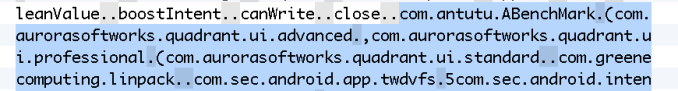
\includegraphics[width=0.8\textwidth,height=1.6cm,keepaspectratio]{s4-twdvfsapp-strings.png}}\\[0.02cm]
  {\footnotesize Strings in the phone's power-management app: AnTuTu, Quadrant, Linpack}\\[0.12cm]
  \uncover<2->{%
  \condtag{midgray}{Precision cut silently}\hspace{0.1cm}\condtag{midgray}{Work skipped on test inputs}\hspace{0.1cm}\condtag{RedLine}{Fingerprinting: the Galaxy S4}}
  \mlsyscredit{Klug and Lal Shimpi, AnandTech, July 30, 2013 (Internet Archive): throughput table (bars), the article's TwDVFSApp screenshot (cropped). Benchmarking, \S12.8.4.}
  \note{[2.5 min] Goodhart's law acting on a company. Step 1: AnandTech measured an international Samsung Galaxy S4 in July 2013. In every game, including the most demanding, its GPU ran at \val{s4_game_mhz} MHz. Under GLBenchmark 2.5.1, AnTuTu, and Quadrant it ran at \val{s4_bench_mhz} MHz. GFXBench 2.7 runs the same low-level triangle test as GLBenchmark 2.5.1, confirmed with the benchmark's makers, and the two results differed by \val{s4_gain} percent: \val{s4_gfx} against \val{s4_glb} million triangles per second. Point to the screenshot, the article's own: AnandTech ran strings on the phone's power-management app, TwDVFSApp, and found benchmark package names (AnTuTu, Quadrant, Linpack) near the string ``BenchmarkBooster.'' The highlighted text is what the investigators highlighted. Step 2: the chapter's three shortcuts that MLPerf's rules forbid: lowering precision without saying so, skipping work the fixed test inputs do not need, and detecting the benchmark to run special settings. The Galaxy S4 is the third. ENGAGE: the higher clock was real hardware. Why is this a problem? Expected: the benchmark predicts game performance only if it runs at the clock games get. FLEX: [CORE]. Samsung said \val{s4_max_mhz} MHz was the maximum and that games ran lower, as reported at the time; the article does not report Samsung's reason.}
\end{frame}

\begin{frame}{A fresh test set shows whether a score was earned}
  \begin{columns}[T]
    \begin{column}{0.58\textwidth}
      \centering{\small\textbf{Lecture 1's ImageNetV2, read for rank}}\\[0.05cm]
      \safeimg[width=\textwidth,height=5.2cm,keepaspectratio]{recht.pdf}
    \end{column}
    \begin{column}{0.38\textwidth}
      \centering{\small\textbf{New grade-school math}}\\[0.05cm]
      \safeimg[width=\textwidth,height=5.2cm,keepaspectratio]{gsm1k.pdf}
    \end{column}
  \end{columns}
  \mlsyscredit{Measured: Recht et al., ICML 2019, appendix table (MatchedFrequency, top-1; their Figure 1 data). Zhang et al., GSM1k, NeurIPS 2024 (abstract).}
  \note{[2.5 min] Two ways a reused test set can stop measuring. Left: Lecture 1's ImageNetV2 scatter, read for a new question. Every model fell \val{recht_lo} to \val{recht_hi} points, yet the dots form a nearly straight line; the rank correlation between old and new accuracy is \val{recht_rho}, so gains on the old set carried over to the new one. The authors attribute the drop to harder images and find little sign of tuning on the old test set. Right: Zhang and colleagues wrote GSM1k, new grade-school math problems matched to the GSM8k benchmark. Some model families lost up to \val{gsm1k_drop} percent, with signs of overfitting at almost every model size, and a model's tendency to reproduce GSM8k examples predicted its gap. ENGAGE: which of the two drops is Goodhart's law? Expected: the right panel, memorization of a public test set; the left is a harder sample with the measure intact. The chapter's defenses: held-out or temporal test sets, sets rebuilt by the original procedure, and contamination checks. FLEX: [CORE].}
\end{frame}

\begin{frame}{Discuss: what would you do for a leaderboard bonus?}
  \mlsysactivity{Discuss}{2 min}
  \centering
  {\large Your team's bonus depends on a public leaderboard rank.}\\[0.25cm]
  {\normalsize Name one change that raises the rank and hurts your users,\\and one rule that would stop it. Two minutes with a neighbor.}\\[0.5cm]
  \uncover<2->{%
    \condtag{BlueLine}{Run rules}\hspace{0.15cm}\condtag{BlueLine}{Latency in the score}\\[0.15cm]
    \condtag{OrangeLine}{Disclosure and audits}\hspace{0.15cm}\condtag{OrangeLine}{Fresh test sets}\\[0.25cm]
    {\small Each rule protects measurement validity, so the score still measures what users get.}}
  \mlsyscredit{Benchmarking, \S12.8.4 (benchmark engineering, bias and over-optimization).}
  \note{[2.5 min] ENGAGE: two minutes, then take three answers. Expected changes: a wider beam or a larger batch that breaks the latency objective (Example 12.1); kernels padded to the benchmark's fixed shapes that fall back to slow paths on real inputs; detecting the benchmark (Galaxy S4); quantizing until the model's confidence is no longer trustworthy; tuning on the public test set. Step 2: the defenses the chapter names. Run rules with a closed division; a latency objective inside the score, as MLPerf's Server scenario does; published compiler flags, kernel configurations, and audits; and test sets the team never saw. WARN: students may conclude that benchmarks are useless. The chapter's point is narrower. A score stays a measure only while rules and fresh data keep it one. Land the segment: a score that becomes the target rewards whatever raises the score. FLEX: [CORE].}
\end{frame}

% =============================================================================
% SECTION: MODEL QUALITY
% =============================================================================
\mlsysnote{[0.5 min] The system half is done. Now the model. The camera trap's INT8 MobileNetV2 is faster on the board, but is it still right, and does it ship? FLEX: [CORE].}
\mlsysdivider{Is the model still right, and does it ship?}{Benchmarking, \S12.9.1, \S12.9.2, \S12.9.3}
\section{Model Quality}

\begin{frame}{Predict: which phone models would you never ship?}
  \mlsysactivity{Predict}{1 min}
  \begin{columns}[T]
    \begin{column}{0.68\textwidth}
      \centering
      \mlsyssteps[width=\textwidth,height=4.9cm,keepaspectratio]{pareto_step}{2}
    \end{column}
    \begin{column}{0.30\textwidth}
      \centering
      \safeimg[width=\textwidth,height=2.4cm,keepaspectratio]{google-pixel-2016.jpg}\\[0.05cm]
      {\footnotesize Google Pixel and Pixel XL (2016); timed: the Pixel}\\[0.25cm]
      \raggedright
      \only<1|handout:0>{\footnotesize Whatever your latency budget, which would you never ship?}%
      \only<2-|handout:1>{\footnotesize Dominated: another model is at least as good on both axes.}
    \end{column}
  \end{columns}
  \mlsyscredit{Measured: Sandler et al., ``MobileNetV2,'' CVPR 2018, Table 4 (Pixel 1, one large core, TF-Lite). Photo: Maurizio Pesce (CC BY 2.0), Wikimedia Commons.}
  \note{[2.5 min] Four ImageNet models timed on one phone CPU core by the MobileNetV2 authors; the phone is the first Google Pixel, shown beside its larger sibling. ENGAGE: whatever your latency budget, which would you never ship? Step 2: MobileNetV1 (\val{sd_mobilenetv1_top1} percent at \val{sd_mobilenetv1_ms} ms) is beaten on both axes by MobileNetV2 (\val{sd_mobilenetv2_top1} percent at \val{sd_mobilenetv2_ms} ms). NASNet-A (\val{sd_nasneta_top1} percent at \val{sd_nasneta_ms} ms) is beaten on both by the wider MobileNetV2 1.4 (\val{sd_mobilenetv214_top1} percent at \val{sd_mobilenetv214_ms} ms). Both are dominated. The two MobileNetV2 points form the Pareto frontier, and choosing between them is a trade of accuracy against latency. WARN: being on the frontier does not mean meeting the deployment's floor; the camera trap's \val{frame_budget} ms frame deadline from Lecture 12 rules out both points on this phone. FLEX: [CORE].}
\end{frame}

\begin{frame}{On another processor of the same phone, the ranking flips}
  \centering
  \safeimg[width=0.95\textwidth,height=5.3cm,keepaspectratio]{lottery.pdf}
  \mlsyscredit{Measured: Chu et al., ``Discovering Multi-Hardware Mobile Models via Architecture Search,'' CVPRW 2021, Table 1 (Pixel 4). Hardware lottery: Benchmarking, \S12.8.3, Figure 10.}
  \note{[1.5 min] One panel of the chapter's hardware-lottery figure, redrawn from the paper's table. Four models of nearly equal accuracy (\val{chu_top1_lo} to \val{chu_top1_hi} percent) on two processors of one Pixel 4. On the CPU in floating point, MobileNetV3 Large is fastest at \val{chu_v3_cpu} ms and MobileNetV1 third at \val{chu_v1_cpu}. On the phone's digital signal processor, MobileNetV1 is fastest at \val{chu_v1_dsp} ms and MobileNetV3 Large third at \val{chu_v3_dsp}. ENGAGE: a team picks MobileNetV3 from a CPU benchmark and ships on the DSP. What did the benchmark tell them? Expected: the wrong ranking. WARN: a frontier measured on one processor does not transfer; measure on the target path (\S12.8.3). FLEX: [OPTIONAL].}
\end{frame}

\begin{frame}{ECE is the average gap between confidence and accuracy}
  \begin{columns}[c]
    \begin{column}{0.50\textwidth}
      \centering\mlsyssteps[width=\textwidth,height=5.8cm,keepaspectratio]{ece_step}{3}
    \end{column}
    \begin{column}{0.48\textwidth}
      \small
      \textbf{Quality beyond accuracy:} is the confidence right?\\[0.3cm]
      $\text{ECE} = \displaystyle\sum_{i} \frac{|\text{bin}_i|}{n}\,\bigl|\text{acc}_i - \text{conf}_i\bigr|$\\[0.3cm]
      \calcline{2}{gaps: \val{bin1_gap}, \val{bin2_gap}, \val{bin3_gap}}
      \calcline{3}{weights: \val{bin1_n}, \val{bin2_n}, \val{bin3_n} of \val{bins_total} predictions}
      \calcline{3}{$\val{bin1_w} \times \val{bin1_gap} + \val{bin2_w} \times \val{bin2_gap} + \val{bin3_w} \times \val{bin3_gap} = \val{ece}$}
    \end{column}
  \end{columns}
  \mlsyscredit{Benchmarking, \S12.9.1, equation 4 (Pakdaman Naeini et al. 2015). Bins constructed for this slide.}
  \note{[3 min] A well-calibrated model that says 80 percent is right about 80 percent of the time. Step 1: a reliability diagram for \val{bins_total} predictions, grouped by confidence into three bins. The \val{bin1_n} predictions near \val{bin1_conf} confidence were right \val{bin1_acc_pct} percent of the time; the \val{bin2_n} near \val{bin2_conf}, \val{bin2_acc_pct} percent; the \val{bin3_n} near \val{bin3_conf}, only \val{bin3_acc_pct} percent. The dashed line is perfect calibration. Step 2: the gap in each bin, shaded: \val{bin1_gap}, \val{bin2_gap}, \val{bin3_gap}. The model is overconfident, most in its most confident bin. Step 3: expected calibration error (ECE) weights each gap by the bin's share of predictions: \val{bin1_w} times \val{bin1_gap} plus \val{bin2_w} times \val{bin2_gap} plus \val{bin3_w} times \val{bin3_gap}, about \val{ece}. That is the size of the INT8 model's ECE in the chapter's camera-trap table. ENGAGE: why does this matter for the camera trap? Expected: if it only alerts above \val{alert_conf} percent confidence, an overconfident model sends wrong alerts it should have held back. WARN: the calibration of quantization ranges in Lecture 10b is a different procedure with the same name. ECE also depends on the number of bins, so a protocol must fix the estimator before comparing models. FLEX: [CORE].}
\end{frame}

\begin{frame}{The more accurate network was three times worse calibrated}
  \centering
  \mlsyssteps[width=0.95\textwidth,height=4.8cm,keepaspectratio]{guo_step}{2}\\[0.05cm]
  \uncover<2->{\small Temperature scaling divides the logits by one fitted constant, so the top class never changes.}
  \mlsyscredit{Measured: Guo, Pleiss, Sun, Weinberger, ``On Calibration of Modern Neural Networks,'' ICML 2017, Figure 1 and Table 1 (15 bins).}
  \note{[2 min] Measured calibration. Step 1: Guo and colleagues compared a 1998 network, LeNet 5, with a 2016 ResNet-110 on CIFAR-100. The ResNet makes fewer errors, \val{guo_resnet_err} against \val{guo_lenet_err} percent, and its ECE is \val{guo_resnet_ece} percent against \val{guo_lenet_ece}, more than three times worse. Accuracy and confidence are separate measurements. Step 2: the fix they found most effective on vision tasks, temperature scaling. Divide the logits (the scores before the softmax) by one constant fitted on held-out data. On ImageNet, ResNet-152's ECE fell from \val{guo_in_ece} to \val{guo_in_ece_ts} percent. Dividing every score by the same positive number cannot change which class is largest, so accuracy is unchanged. ENGAGE: could temperature scaling fix a model that misses rare species at night? Expected: no; it changes confidence and leaves the winning class alone. FLEX: [OPTIONAL]; cutting it loses the measured calibration comparison.}
\end{frame}

\begin{frame}{On unseen camera traps, macro F1 fell \val{wilds_f1_drop_int} points, accuracy \val{wilds_acc_drop_int}}
  \begin{columns}[T]
    \begin{column}{0.45\textwidth}
      \centering
      \safeimg[width=\textwidth,height=5.4cm,keepaspectratio]{wilds.pdf}
    \end{column}
    \begin{column}{0.53\textwidth}
      \centering
      {\footnotesize\textbf{A training trap}\hfill\textbf{An unseen trap}}\\[0.05cm]
      \safeimg[width=\textwidth,height=5.7cm,keepaspectratio]{wilds-iwildcam-traps.png}
    \end{column}
  \end{columns}
  \mlsyscredit{Measured: Koh et al., ``WILDS,'' ICML 2021, Table 4 (iWildCam2020-WILDS, ResNet-50, ERM). Images: the paper's iWildCam figure, cropped.}
  \note{[2 min] The camera trap's real risk, measured. Right: real images from the dataset, cropped from the paper's figure. A trap in the training set (location 245) and a trap the model never saw (location 246): new background, new light, new species such as the great curassow. WILDS's iWildCam split trains a ResNet-50 species classifier on photos from one set of camera traps and tests it on traps it has never seen, where the background, light, and mix of species change. Average accuracy falls \val{wilds_acc_drop} points, from \val{wilds_id_acc} to \val{wilds_ood_acc} percent, which looks tolerable. Macro F1 averages the F1 score of each species equally, so rare species count as much as common ones; it falls \val{wilds_f1_drop_int} points, from \val{wilds_id_f1} to \val{wilds_ood_f1}. Error bars are the standard deviation over \val{wilds_reps} runs. F1 combines precision (the fraction of predicted sightings that are right) and recall (the fraction of real sightings found). ENGAGE: why does the average hide the loss? Expected: common species dominate the image count. In the chapter's version, a classifier can be 99 percent accurate and find one rare animal in ten (illustrative). LINK: Lecture 15 builds release gates on per-group results. The chapter's Camelyon17 case shows the same drop across hospitals, \val{camelyon_id} to \val{camelyon_ood} percent. FLEX: [CORE].}
\end{frame}

\begin{frame}{Diagnose: top-1 passes, ECE fails, edge cases open}
  \mlsysactivity{Diagnose}{2.5 min}
  \centering\footnotesize
  \begin{tabular}{@{}lcccl@{}}
    \toprule
    \textbf{Gate (set before the test)} & \textbf{FP32} & \textbf{INT8} & \textbf{Pass?} & \textbf{Enough data?} \\
    \midrule
    Top-1, loss under \val{g_limit} point & \val{g_top1_fp32}\% & \val{g_top1_int8}\% & \uncover<2->{\textcolor{GreenLine}{\textbf{yes}}} & \uncover<4->{only if the paired interval stays under \val{g_limit}} \\
    Top-5, loss under \val{g_limit} point & \val{g_top5_fp32}\% & \val{g_top5_int8}\% & \uncover<2->{\textcolor{GreenLine}{\textbf{yes}}} & \uncover<4->{same} \\
    ECE, no rise & \val{g_ece_fp32} & \val{g_ece_int8} & \uncover<3->{\textcolor{RedLine}{\textbf{no}}} & \uncover<4->{same estimator, same bins} \\
    Edge cases, no drop & \val{g_edge_fp32}\% & \val{g_edge_int8}\% & \only<3|handout:0>{\textcolor{RedLine}{\textbf{no}}}\only<4-|handout:1>{\colorbox{OrangeLine!20}{\textbf{\textcolor{OrangeLine}{unresolved}}}} & \uncover<4->{\colorbox{RedLine!15}{\val{g_edge_n} images: $\pm$\val{g_edge_hw} points}} \\
    Board latency, energy & \multicolumn{3}{c}{\uncover<4->{measured in Part 1}} & \uncover<4->{stated conditions} \\
    \bottomrule
  \end{tabular}\\[0.2cm]
  {\footnotesize\textcolor{midgray}{Assumed values (chapter scenario). Edge cases: heavy occlusion, low light, rotation; about \val{edge_share_pct}\% of inputs.}}
  \mlsyscredit{Benchmarking, Lighthouse 12.3 and Table 18 (assumed values). Edge-case margin: binomial 95\% at \val{g_edge_fp32_int}\% on \val{g_edge_n} images, derived.}
  \note{[3 min] The chapter's acceptance rule for the camera trap's INT8 MobileNetV2, set before compression: less than \val{g_limit_words} point of top-1 or top-5 loss, no rise in ECE, no drop on edge cases. The values are assumed. ENGAGE: ship it, and is there enough data to tell? Step 2: top-1 and top-5 pass on their point estimates. Step 3: ECE triples, from \val{g_ece_fp32} to \val{g_ece_int8}, and edge-case accuracy falls \val{g_edge_drop} points. On the point estimates, both fail. Step 4: apply segments 1 and 2. A \val{g_top1_loss}-point drop passes only if the paired interval stays below \val{g_limit} point, which needs per-image outcomes. Edge cases are about \val{edge_share_pct} percent of inputs: about \val{g_edge_n} in a \val{g_test}-image test, so \val{g_edge_fp32_int} percent is known only to about plus or minus \val{g_edge_hw} points. So the edge-case cell turns from no to unresolved. ECE alone fails, and the edge-case gate needs more edge cases. The next frame names this gap. WARN: temperature scaling may repair the ECE but cannot change which class wins; edge-case errors need a diagnosis of quantization ranges and data (in the chapter, ranges calibrated on ImageNet clip night-time infrared frames). LINK: Lecture 14 owns the online gate: shadow, canary, A/B tests, rollback. FLEX: [CORE].}
\end{frame}

\begin{frame}[t]{Verification gap: a test set samples almost no inputs}
  \mlsysactivity{Estimate}{1.5 min}
  \centering
  {\normalsize How many different \val{img_w} $\times$ \val{img_h} color images with \val{img_bits}-bit pixels exist?}\\[0.35cm]
  \raggedright\hspace{1.2cm}\begin{minipage}{0.8\textwidth}\small
  \calcline{2}{Values per image: $\val{img_w} \times \val{img_h} \times \val{img_c} = \val{img_values}$, each one of \val{img_levels}}
  \calcline{2}{Possible images: $\val{img_levels}^{\val{img_values}} \approx 10^{\val{space_exp}}$}
  \calcline{3}{ImageNet validation set: $\val{test_n} \approx 10^{\val{test_exp}}$ images}
  \calcline{3}{Fraction a test set covers: about $10^{-\val{frac_exp}}$}
  \end{minipage}\\[0.3cm]
  \centering
  \uncover<4->{\normalsize A passed test certifies the population it sampled,\\within the margin its size allows. Nothing else.}
  \mlsyscredit{Benchmarking, \S12.9 (the verification gap: a test set covers an effectively zero fraction of the input space). Counts derived.}
  \note{[2 min] ENGAGE: one minute; an order of magnitude is enough. Step 2: an image is \val{img_w} by \val{img_h} pixels by \val{img_c} colors, \val{img_values} values, each one of \val{img_levels} levels, so there are \val{img_levels} to the power \val{img_values} possible images, about 10 to the \val{space_exp}. Step 3: a \val{test_n}-image test set covers about 10 to the minus \val{frac_exp} of that space; effectively zero. Step 4: the chapter's verification gap. A test never certifies a model on all inputs; it certifies behavior on the population it sampled, within the uncertainty its size allows. That is why the previous slide's edge-case gate is unresolved and why the camera trap at a new site fell \val{wilds_f1_drop_int} points of macro F1. WARN: students conclude testing is pointless. Most of those images are noise no camera will produce; the defense samples the deployment's population, its slices, and its drift, since no test can cover the space. LINK: Lecture 14b monitors the population after release. FLEX: [CORE].}
\end{frame}

% =============================================================================
% CLOSE
% =============================================================================
\begin{frame}[t]{The gap is real, unattributable, and too small to use}
  \mlsysactivity{Retrieval}{2 min}
  \centering
  \safeimg[width=0.8\textwidth,height=3.5cm,keepaspectratio]{hook_step2.pdf}\\[0.15cm]
  \only<1|handout:0>{\normalsize Close your notes. Write the three questions you would ask before saying one server is faster.}%
  \only<2|handout:0>{%
    \condtag{GreenLine}{Real: excludes zero}\hspace{0.1cm}%
    \condtag{RedLine}{Not attributable}\hspace{0.1cm}%
    \condtag{RedLine}{Not useful: under \val{min_useful}\%}\\[0.12cm]
    {\small Interval \val{pct_lo_dell} to \val{pct_hi_dell}\%; host and software changed too. H200: same host and software, \val{pct_lo_h200} to \val{pct_hi_h200}\% faster.}}%
  \only<3-|handout:1>{%
    \condtag{BlueLine}{Load and statistic}\hspace{0.1cm}\condtag{BlueLine}{Boundary}\hspace{0.1cm}\condtag{OrangeLine}{Scenario}\\[0.1cm]
    \condtag{OrangeLine}{Power and heat}\hspace{0.1cm}\condtag{RedLine}{Noise: runs, samples}\hspace{0.1cm}\condtag{RedLine}{Quality held}}
  \mlsyscredit{MLPerf Training v4.0 (intervals derived). Conditions: Lectures 12 and 12b.}
  \note{[2.5 min] Back to the two servers. ENGAGE: close your notes, one minute, write the three questions. Step 2: is the gap larger than its noise? Yes: the interval, \val{pct_lo_dell} to \val{pct_hi_dell} percent, excludes zero. Did one thing change? No: the host CPU, host memory, software container, operating system, and driver also differ, so the gap belongs to the whole submission. Is it worth acting on? No: it is below a \val{min_useful} percent threshold set in advance, and one of Dell's five runs never reached the quality target. The H200 server kept Eos's host and software, changed the accelerator, and is \val{pct_h200} percent faster, interval \val{pct_lo_h200} to \val{pct_hi_h200}: real, attributable to the accelerator with the driver as the one caveat, and useful. Step 3: with Part 1's four conditions, a benchmark claim now states six: the load and statistic, the boundary, the scenario, the power boundary and heat, the noise, and the quality held. For a model, the last one expands into today's gates: the frontier on the target processor, calibration, the slices that matter, and enough data to tell. That last clause is the chapter's Verification Gap. A passed test is evidence about the population it sampled and proves nothing about deployment. FLEX: [CORE].}
\end{frame}

\begin{frame}{Takeaways}
  \thumbline{thumb_strip_step2.pdf}{Measure the noise before comparing. A suite fixes how many runs it takes and how they combine.}\\[0.12cm]
  \thumbline{thumb_interval_step5.pdf}{A difference needs an interval that excludes zero, one change, and a threshold set first.}\\[0.12cm]
  \thumbline{thumb_fingerprint.pdf}{A score that becomes the target needs run rules, disclosure, and fresh test sets.}\\[0.12cm]
  \thumbline{thumb_wilds.pdf}{A model ships on its frontier, calibration, and slices, with enough data in each. A passed test is evidence about the population it sampled.}
  \note{[1 min] One line per segment; each thumbnail is the figure that taught it. Ask students to star the line they would have gotten wrong before today. FLEX: [CORE].}
\end{frame}

\begin{frame}{Open questions}
  \normalsize
  \begin{itemize}\setlength{\itemsep}{0.35cm}
    \item Static test sets saturate and leak into training data; dynamic ones cannot be compared across years. For a product shipping next year, which would you trust, and why?
    \item Who should set the minimum useful difference for a hardware purchase or a model swap: engineering, finance, or product? Why before the measurement?
    \item The camera trap passes every lab gate. What is the cheapest field measurement that shows it still works at night, at a new trap, a year later?
  \end{itemize}
  \note{[0.5 min] No single answer. Take one response to each if time allows, or assign one as a short written response. For the first, the chapter's dataset-saturation figure shows benchmarks crossing human baselines within a few years, and Dynabench-style dynamic sets are one answer. For the second, the threshold encodes the cost of switching, which engineering alone does not know. For the third, students should name a small labeled field sample and a monitored statistic; Lecture 14b owns monitoring. FLEX: [OPTIONAL].}
\end{frame}

\begin{frame}{Read and explore}
  \small
  \begin{itemize}\setlength{\itemsep}{0.06cm}
    \item \textbf{Read:} Benchmarking, \S12.8.1 to \S12.8.4, \S12.9.1 to \S12.9.3, \S12.10, \S12.11 (Table 21); Napkin Math 12.5 and Lighthouse 12.3.
    \item \textbf{Practice:} recompute today's interval from the ten logged runs; train a small CIFAR-10 model with five seeds, and report the spread and ECE before and after temperature scaling.
    \item MLCommons, MLPerf Training rules (scoring) and Inference rules (query counts).
    \item Guo et al., ``On Calibration of Modern Neural Networks,'' ICML 2017.
    \item Koh et al., ``WILDS: A Benchmark of in-the-Wild Distribution Shifts,'' ICML 2021.
    \item Zhang et al., ``A Careful Examination of Large Language Model Performance on Grade School Arithmetic,'' NeurIPS 2024.
  \end{itemize}
  \note{[0.5 min] The chapter first, with its self-check questions for \S12.8 and \S12.9. The run logs are public in the mlcommons/training\_results\_v4.0 repository; recomputing the interval takes fifteen minutes and makes the worked example concrete. The MLPerf rules show how a community turns noisy runs into one score. Guo et al. is short and explains reliability diagrams and temperature scaling. WILDS measures the camera-trap and hospital shifts. Zhang et al. shows how to build a fresh test set to measure memorization. For students who want more on seeds, Henderson et al. (AAAI 2018) shows seeds reversing published comparisons in reinforcement learning. FLEX: [OPTIONAL].}
\end{frame}

\begin{frame}[c]
  \begin{columns}[c]
    \begin{column}{0.58\textwidth}
      {\small\textcolor{lightgray}{NEXT LECTURE \textbar{} MODEL SERVING, PART 1}}\\[0.5cm]
      {\LARGE\bfseries The model passed its gates in the lab. What changes when real users send requests?}
    \end{column}
    \begin{column}{0.38\textwidth}
      \centering\mlsysphoto[width=\textwidth,height=4.2cm,keepaspectratio]{nvidia-h100-pcie.jpg}\\[0.05cm]{\footnotesize An NVIDIA H100, the accelerator Lecture 13 serves on}
    \end{column}
  \end{columns}
  \mlsyscredit{Photo: NVIDIA H100 PCIe, Geekerwan (CC BY 3.0), Wikimedia Commons.}
  \note{[0.5 min] Close on Lecture 13's question. Both parts of this lecture measured under fixed, stated conditions. Next time the load is real users arriving at random, and the serving system decides the batch size and the queue that create the tail. FLEX: [CORE].}
\end{frame}

\end{document}
